
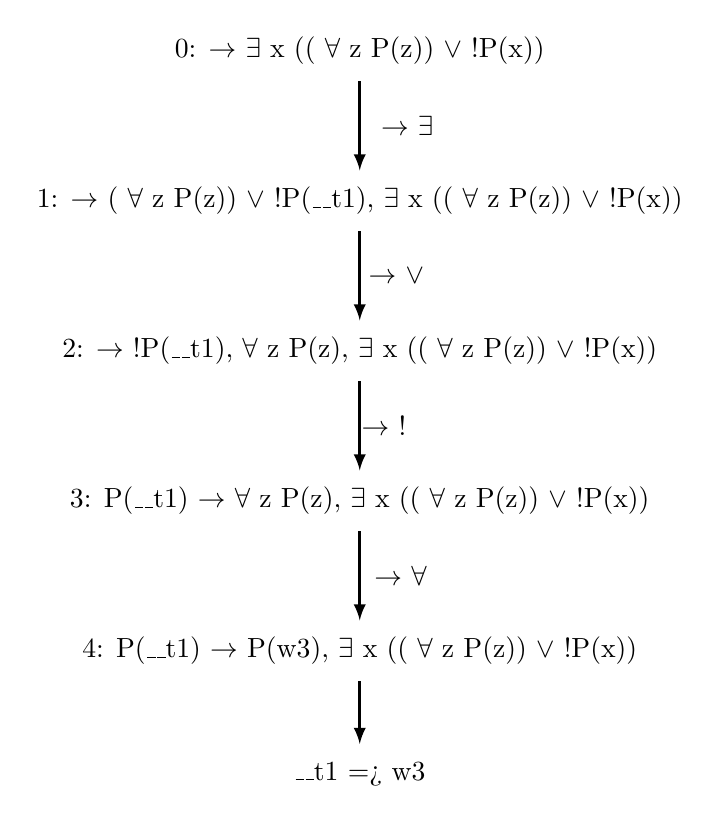
\begin{tikzpicture}[>=latex,line join=bevel,scale=0.60]
  \pgfsetlinewidth{1bp}
%%
\pgfsetcolor{black}
  % Edge: 0 -> 1
  \draw [->] (231bp,433.79bp) .. controls (231bp,421.34bp) and (231bp,404.61bp)  .. (231bp,380.19bp);
  \definecolor{strokecol}{rgb}{0.0,0.0,0.0};
  \pgfsetstrokecolor{strokecol}
  \draw (259.5bp,407bp) node {$\rightarrow$  $\exists$};
  % Edge: 4 -> 5
  \draw [->] (231bp,73.708bp) .. controls (231bp,65.464bp) and (231bp,55.538bp)  .. (231bp,36.082bp);
  % Edge: 3 -> 4
  \draw [->] (231bp,163.79bp) .. controls (231bp,151.34bp) and (231bp,134.61bp)  .. (231bp,110.19bp);
  \draw (255.5bp,137bp) node {$\rightarrow$ $ \forall$};
  % Edge: 1 -> 2
  \draw [->] (231bp,343.79bp) .. controls (231bp,331.34bp) and (231bp,314.61bp)  .. (231bp,290.19bp);
  \draw (253bp,317bp) node {$\rightarrow$ $\vee$};
  % Edge: 2 -> 3
  \draw [->] (231bp,253.79bp) .. controls (231bp,241.34bp) and (231bp,224.61bp)  .. (231bp,200.19bp);
  \draw (245.5bp,227bp) node {$\rightarrow$ !};
  % Node: 1
\begin{scope}
  \definecolor{strokecol}{rgb}{0.0,0.0,0.0};
  \pgfsetstrokecolor{strokecol}
  \draw (231bp,362bp) node {1:   $\rightarrow$ ( $ \forall$ z P(z)) $\vee$ !P(\_\_t1),  $\exists$ x (( $ \forall$ z P(z)) $\vee$ !P(x))};
\end{scope}
  % Node: 0
\begin{scope}
  \definecolor{strokecol}{rgb}{0.0,0.0,0.0};
  \pgfsetstrokecolor{strokecol}
  \draw (231bp,452bp) node {0:   $\rightarrow$  $\exists$ x (( $ \forall$ z P(z)) $\vee$ !P(x))};
\end{scope}
  % Node: 3
\begin{scope}
  \definecolor{strokecol}{rgb}{0.0,0.0,0.0};
  \pgfsetstrokecolor{strokecol}
  \draw (231bp,182bp) node {3:  P(\_\_t1) $\rightarrow$  $ \forall$ z P(z),  $\exists$ x (( $ \forall$ z P(z)) $\vee$ !P(x))};
\end{scope}
  % Node: 2
\begin{scope}
  \definecolor{strokecol}{rgb}{0.0,0.0,0.0};
  \pgfsetstrokecolor{strokecol}
  \draw (231bp,272bp) node {2:   $\rightarrow$ !P(\_\_t1),  $ \forall$ z P(z),  $\exists$ x (( $ \forall$ z P(z)) $\vee$ !P(x))};
\end{scope}
  % Node: 5
\begin{scope}
  \definecolor{strokecol}{rgb}{0.0,0.0,0.0};
  \pgfsetstrokecolor{strokecol}
  \draw (231bp,18bp) node {\_\_t1 => w3};
\end{scope}
  % Node: 4
\begin{scope}
  \definecolor{strokecol}{rgb}{0.0,0.0,0.0};
  \pgfsetstrokecolor{strokecol}
  \draw (231bp,92bp) node {4:  P(\_\_t1) $\rightarrow$ P(w3),  $\exists$ x (( $ \forall$ z P(z)) $\vee$ !P(x))};
\end{scope}
%
\end{tikzpicture}

